\documentclass[acmsmall,nonacm]{acmart}

% Tables
\usepackage{array}
\usepackage{tabularx}
\usepackage{tikz}
\usetikzlibrary{arrows.meta,positioning}

% ACM journal configuration
\acmJournal{CSUR}
\citestyle{acmauthoryear}
\settopmatter{printacmref=false}

\title{Comparing AI-Assisted and Manual Data Labelling Accuracy on Scientific Datasets}
\subtitle{A Review and Comparative Analysis of Annotation Quality in Scientific and Biomedical Machine Learning Pipelines}
\author{Ujjwal Nikam}
\affiliation{%
  \institution{IIIT Allahabad}
  \country{\relax}
}

\begin{document}

\begin{abstract}
High-quality labelled data underpins the training and evaluation of virtually every supervised machine learning system used in scientific research, from biomedical literature screening to medical image segmentation and astronomical classification. As large language models (LLMs) and other AI-assisted tools have matured, researchers increasingly rely on them to accelerate or partially replace manual annotation. This paper reviews and synthesises empirical evidence comparing the accuracy of AI-assisted and purely manual data labelling on scientific datasets. Drawing on studies spanning text annotation, systematicreview screening, medical image segmentation, and figure/metadata extraction, we find that AI-assisted and hybrid human-in-the-loop pipelines frequently match or exceed the accuracy of unaided manual annotation on well-defined, structured tasks, while manual annotation retains an advantage on ambiguous, high-context, or safety-critical judgements. We further discuss automation bias, benchmark label-error rates, active-learning strategies for reducing annotation cost, and current tooling, before identifying open research gaps --- including the scarcity of large-scale, domain-diverse accuracy comparisons on genuinely scientific (as opposed to social-media or general web) datasets --- and proposing directions for future work.
\end{abstract}

\keywords{Data labelling; data annotation; artificial intelligence; large language models; human-in-the-loop; active learning; label quality; scientific datasets; crowdsourcing; automation bias.}

\nocite{alathba2026cohesion,chelli2024hallucination,chen2025human,chen2024quality,delgadochaves2025large,dreizin2023accelerating,gilardi2023chatgpt,khraisha2023large,mahmoudi2025critical,northcutt2021pervasive,northcutt2021confident,settles2009active,siegel2018extracting,turner2025large,validation2025llama,yamagata2024survey}

\maketitle

\section{Introduction}
\label{sec:introduction}

Supervised machine learning models are only as reliable as the labels on which they are trained and evaluated. In scientific domains --- biomedical imaging, systematic literature review, neuroimaging metadata curation, and figure or table extraction from scholarly documents --- labelled data is simultaneously indispensable and expensive to produce, because it typically requires domain expertise that general-purpose crowdsourcing platforms cannot supply. Traditionally, manual annotation by trained experts or research assistants has been treated as the gold standard against which automated methods are judged, yet manual annotation is slow, costly, and itself imperfect: even careful two-reviewer screening in systematic reviews misses a measurable share of relevant records, and single-reviewer screening misses substantially more.

The emergence of capable large language models such as GPT-4 and its successors has changed this calculus. A growing body of work shows that LLM-based annotation can match or exceed the accuracy of non-expert crowd workers on text-classification tasks, and can perform comparably to trained human annotators on some scientific metadata-extraction tasks. At the same time, other studies report substantial variability in LLM accuracy across biomedical domains, and highlight risks such as hallucinated citations and a psychological automation bias in which human reviewers over-trust AI-generated prelabels and reduce their own scrutiny.

This paper synthesises the empirical literature comparing AI-assisted and manual data labelling accuracy specifically in scientific contexts. Section~\ref{sec:background} reviews related work and establishes the conceptual background. Section~\ref{sec:main-discussion} presents a thematic and technical discussion of the mechanisms by which AI assistance changes labelling accuracy. Section~\ref{sec:current-approaches} surveys current tools and workflows. Section~\ref{sec:challenges} discusses methodological challenges and limitations in the evidence base itself. Section~\ref{sec:future-directions} identifies research gaps and future directions, and Section~\ref{sec:conclusion} concludes.

\section{Background and Related Work}
\label{sec:background}

\subsection{Manual annotation: strengths and structural costs}
\label{subsec:manual-annotation}

Manual annotation by trained personnel has long been treated as the reference standard for supervised learning because human experts can draw on contextual, cultural, and domain knowledge that purely statistical systems lack. This strength is clearest on ambiguous material. In a controlled comparison of manual and ChatGPT-assisted annotation of Arabic social-media discourse, manual annotation excelled at identifying nuanced expressions such as sarcasm and cultural references, achieving 90--94\% accuracy against a goldstandard reference set, compared with 82--87\% for unverified AI output on the same items \citep{alathba2026cohesion}. The same study, however, documents the structural cost of manual work: the process was time-intensive and mentally demanding, with a risk of annotator fatigue and subjective bias \citep{alathba2026cohesion}. The evidence therefore distinguishes the contextual strength of trained human judgement from the assumption that all forms of manual annotation, including expert and crowd annotation, are equally accurate or consistent.

In biomedical evidence synthesis, the cost of manual annotation is especially visible. Even when two reviewers resolve disagreements through discussion, up to about 3\% of relevant citations can be missed during screening, and single-reviewer screening --- often used to save time in rapid reviews --- can miss as many as 13\% of relevant publications (see discussion in the JAMIA review of LLM-assisted systematic reviews). Inter-reader reliability between human screeners in systematic reviews is also inconsistent, with reported kappa values ranging from roughly 0.37 to 0.90 depending on the review and the reviewers involved. These figures indicate that ``manual'' is not synonymous with ``error-free'': human annotation quality depends heavily on annotation schema design, quality-assurance rigor, and disagreementresolution strategy rather than being a fixed property of human judgement.

Taken together, these studies agree that manual annotation remains particularly valuable when labels require contextual interpretation or expert adjudication. At the same time, they show that its accuracy and consistency are conditional on annotator expertise, reviewer agreement, and quality-control procedures, while its time and labour requirements limit throughput. Manual annotation is therefore an important comparator for AI-only and hybrid approaches, but not an error-free ground truth by definition.

\subsection{The rise of AI-assisted and LLM-based annotation}
\label{subsec:ai-assisted-annotation}

AI-only annotation has shown its clearest advantages on structured classification tasks. A landmark comparison by \citet*{gilardi2023chatgpt} evaluated zero-shot ChatGPT annotation against crowd workers on four samples of tweets and news articles ($n = 6{,}183$) across relevance, stance, topic, and frame-detection tasks. They report that the zero-shot accuracy of ChatGPT exceeded that of crowd workers by about 25 percentage points on average, and that ChatGPT's intercoder agreement exceeded that of both crowd workers and trained research-assistant annotators across all tasks, at roughly one-twentieth to one-thirtieth of the per-annotation cost of Amazon Mechanical Turk \citep{gilardi2023chatgpt}. These results connect AI-only annotation with gains in accuracy relative to crowd annotation, consistency across repeated decisions, lower cost, and higher throughput. However, because the study addressed general text-classification tasks rather than scientific datasets narrowly defined, it provides a baseline rather than a general conclusion about scientific annotation.

In more technical scientific settings, results are more mixed. \citet{turner2025large} evaluated GPT-4o on metadata extraction from the human neuroimaging literature and found performance comparable with trained human annotators, reaching agreement scores of 0.91--0.97 on zero-shot prompts, with LLM errors mostly resembling human errors rather than differing qualitatively from them. By contrast, a validation study of Llama 3 70B and ChatGPT-4o mini for title-and-abstract screening in biomedical systematic reviews found lower sensitivity (56--78\%, depending on configuration) alongside high specificity (91--95\%) and overall accuracy around 90--92\% against human decisions on 1,081 articles, showing that AI-assisted screening trades recall for precision in ways that must be tuned rather than assumed \citetext{PMC12623132}. A separate evaluation of 18 LLMs across three clinical domains found classification accuracy ranging from 40\% to 92\%, underscoring substantial variability across models, prompts, and tasks \citep{delgadochaves2025large}. Thus, the scientific-domain studies agree that AI-only systems can produce consistent and efficient labels on well-specified tasks, but they disagree in the level of accuracy achieved across domains and configurations. The contrast with manual annotation is consequently task-dependent rather than uniform.

Hybrid human-in-the-loop approaches address this variability by combining AI-generated labels with human verification. In the Arabic discourse study, verification increased AI-assisted accuracy from 82--87\% before verification to 88--91\% after verification, narrowing the gap with unaided manual annotation while retaining the role of human judgement on ambiguous cases \citep{alathba2026cohesion}. In scientific workflows, \citet{dreizin2023accelerating} incorporate quality assurance and bias mitigation into AI-collaborative medical-image annotation, while \citet{chen2025human} use an explicit human--LLM collaboration protocol for precision-oncology trial screening because unassisted model reliability remains challenging. Across these studies, the area of agreement is that AI can increase throughput and provide consistent candidate labels, whereas human verification remains important when task ambiguity, domain specificity, or error consequences make AI-only output insufficient. The principal disagreement concerns how much verification is required, because the underlying AI accuracy varies substantially by task and model.

\subsection{Label quality as a property of datasets, not just annotators}
\label{subsec:label-quality}

A complementary strand of work shifts the comparison from annotator type to the quality of the resulting dataset. \citeauthor*{northcutt2021pervasive} (2021) algorithmically identified label errors in the testsets of ten widely used computer vision, natural-language, and audio benchmark datasets using confident learning, and validated a random sample of flagged instances via crowdsourcing; they estimate an average of at least 3.3\% label errors across the ten datasets, including approximately 6\% of the ImageNet validation set, and show that these errors are large enough to change the ranking of competing models on standard leaderboards. The associated confident-learning framework \citetext{Northcutt, Jiang, \& Chuang, 2021} provides a general statistical method for estimating uncertainty in given labels by modelling the joint distribution between noisy and true labels, and has since been adopted to correct labels in domain-specific benchmarks such as the Wake Vision TinyML dataset. This work reinforces the manual-annotation findings above: even long-standing ``manually labelled'' gold-standard datasets contain non-trivial, systematic error, so manual labels cannot automatically serve as an unquestioned reference against which AI-only or hybrid approaches are evaluated.

In medical image segmentation specifically, \citet*{chen2024quality} note that public datasets increasingly mix manual expert annotations with AI-generated pseudo-annotations of varying and largely uncontrolled quality, motivating their proposed Quality Sentinel regression model --- trained on over four million image-label pairs --- to automatically estimate label quality across 142 body structures without a systematic, reliable, automatic quality-control process, a gap that previously did not exist in the field. This approach complements human verification by providing a scalable mechanism for identifying labels that require further review, regardless of whether those labels originated from experts or AI systems.

The literature therefore converges on label quality as a property of the complete annotation pipeline rather than of humans or AI alone. It also exposes the central research gap developed in the following sections: direct, matched comparisons of manual, AI-only, and hybrid pipelines remain limited across genuinely scientific domains, and reported results use different tasks, models, quality controls, and accuracy measures. A clearer comparison must consequently examine not only final accuracy, but also consistency, ambiguity, cost, throughput, and the role of human verification.

\section{Main Thematic and Technical Discussion}
\label{sec:main-discussion}

Table~\ref{tab:results} consolidates the comparison among manual annotation, fully automated or AI-only annotation, and hybrid human-in-the-loop annotation across six dimensions reported throughout the literature: accuracy, handling of ambiguous items, throughput, cost, consistency, and characteristic failure modes.

\subsection{Task structure predicts the accuracy gap}
\label{subsec:task-structure}

Across the studies reviewed, the direction and size of the accuracy gap between AI-assisted and manual labelling tracks the structure of the underlying task. On well-defined, rule-governed classification problems --- relevance judgement, topic labelling, structured metadata fields --- AI assistance tends to match or exceed manual accuracy, particularly relative to non-expert crowd workers \citep{gilardi2023chatgpt,turner2025large}. On tasks requiring cultural, pragmatic, or highly contextual judgement --- sarcasm detection, discourse framing, nuanced sentiment in a politically sensitive corpus --- unaided AI output shows a measurable accuracy deficit relative to trained human annotators, on the order of 6--9 percentage points in the Cohesion-6K comparison \citep{alathba2026cohesion}. This pattern is consistent with the broader observation, echoed across the AI-assisted annotation literature, that neither approach is uniformly best: manual annotation is favoured when ambiguity is high, schemas are still evolving, or errors are especially costly, whereas automated approaches are favoured for rigid, high-agreement patterns that can be validated downstream.

The accuracy comparison is therefore inseparable from ambiguous-item handling. Manual expert annotation is strongest where sarcasm, cultural context, or domain nuance must be interpreted, although its accuracy varies across annotators. Fully automated or AI-only labelling is more consistent on repetitive, well-specified decisions and can match or exceed crowd annotation, but it is weaker on edge cases and rare classes. Hybrid annotation combines these strengths by using the model for routine candidate labels and directing uncertain or nuanced cases to human review. As summarised in Table~\ref{tab:results}, the hybrid approach provides the strongest balance when automated consistency can be combined with human interpretation rather than treated as a substitute for it.

Figure~\ref{fig:labelling_taxonomy} shows the taxonomy of scientific data labelling approaches discussed in this review.

\begin{figure}[t]
\centering
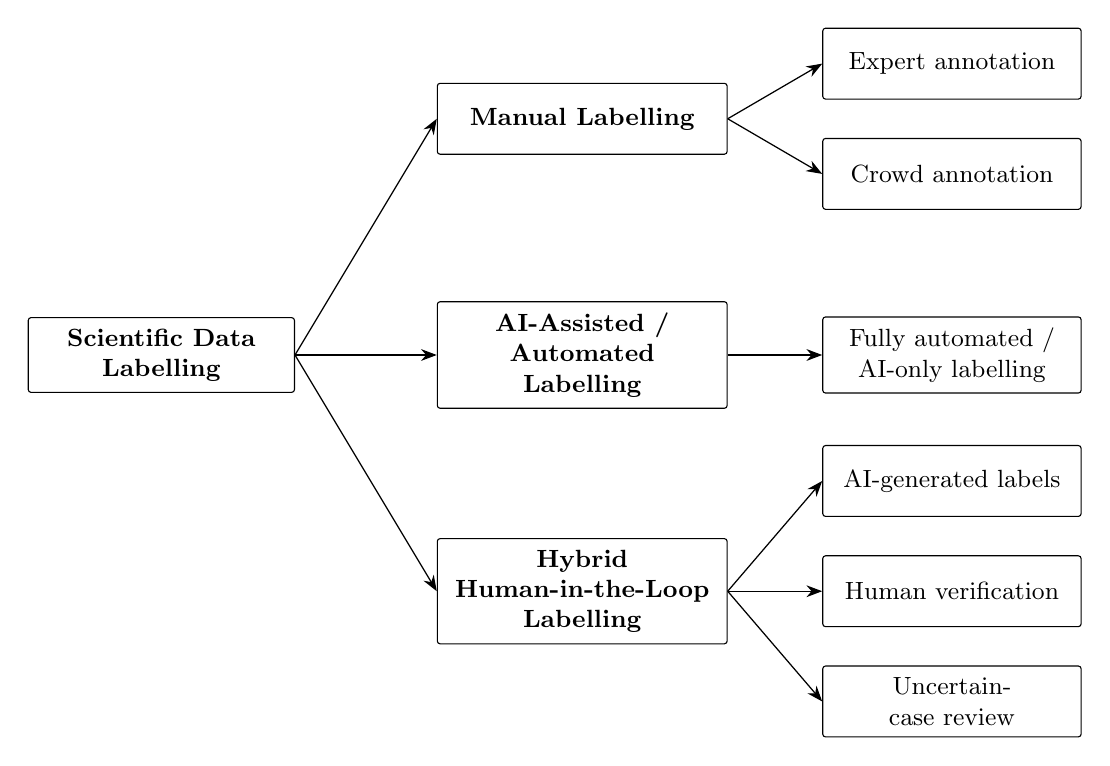
\begin{tikzpicture}[
  node distance=8mm and 12mm,
  >={Stealth[length=2mm]},
  every node/.style={font=\small, align=center},
  taxonomy/.style={draw, rectangle, rounded corners=1pt, minimum height=9mm, inner sep=4pt},
  root/.style={taxonomy, text width=31mm, font=\small\bfseries},
  category/.style={taxonomy, text width=34mm, font=\small\bfseries},
  leaf/.style={taxonomy, text width=30mm},
  link/.style={draw, ->, line width=0.45pt}
]
  \node[root] (root) {Scientific Data Labelling};

  \node[category, right=18mm of root, yshift=30mm] (manual) {Manual Labelling};
  \node[category, right=18mm of root] (automated) {AI-Assisted /\\Automated Labelling};
  \node[category, right=18mm of root, yshift=-30mm] (hybrid) {Hybrid\\Human-in-the-Loop\\Labelling};

  \node[leaf, right=12mm of manual, yshift=7mm] (expert) {Expert annotation};
  \node[leaf, right=12mm of manual, yshift=-7mm] (crowd) {Crowd annotation};

  \node[leaf, right=12mm of automated] (aionly) {Fully automated /\\AI-only labelling};

  \node[leaf, right=12mm of hybrid, yshift=14mm] (ailabels) {AI-generated labels};
  \node[leaf, right=12mm of hybrid] (verification) {Human verification};
  \node[leaf, right=12mm of hybrid, yshift=-14mm] (uncertain) {Uncertain-case review};

  \draw[link] (root.east) -- (manual.west);
  \draw[link] (root.east) -- (automated.west);
  \draw[link] (root.east) -- (hybrid.west);

  \draw[link] (manual.east) -- (expert.west);
  \draw[link] (manual.east) -- (crowd.west);
  \draw[link] (automated.east) -- (aionly.west);
  \draw[link] (hybrid.east) -- (ailabels.west);
  \draw[link] (hybrid.east) -- (verification.west);
  \draw[link] (hybrid.east) -- (uncertain.west);
\end{tikzpicture}
\caption{Taxonomy of scientific data labelling approaches.}
\Description{A taxonomy with scientific data labelling divided into manual labelling, AI-assisted or automated labelling, and hybrid human-in-the-loop labelling. Manual labelling contains expert annotation and crowd annotation. AI-assisted or automated labelling contains fully automated or AI-only labelling. Hybrid human-in-the-loop labelling contains AI-generated labels, human verification, and uncertain-case review.}
\label{fig:labelling_taxonomy}
\end{figure}

\subsection{The hybrid, human-in-the-loop pattern}
\label{subsec:human-in-the-loop}

The most consistent empirical finding across scientific-domain studies is that hybrid pipelines --- in which an AI system proposes labels and a human annotator verifies, corrects, or adjudicates them --- outperform either pure-manual or pure-AI labelling in isolation. In the Cohesion-6K annotation study, AI-assisted accuracy rose from a pre-verification range of 82--87\% to a post-verification range of 88--91\%, closing most, though not all, of the gap to unaided manual annotation, while retaining much of the speed advantage of automation \citep{alathba2026cohesion}. In radiological image annotation, \citet{dreizin2023accelerating} describe an AI-collaborative labeling workflow for voxelwise annotation of trauma CT scans that incorporates explicit quality-assurance and bias-mitigation steps to accelerate the painstaking labeling of targets that vary considerably in volume, addressing a bottleneck that had previously prohibited scaling of data annotation efforts in precision-medicine imaging \citep{dreizin2023accelerating}. In precision-oncology trial screening, \citet{chen2025human} propose a human-LLM collaborative annotation approach precisely because GPT-3.5-class models, used alone, offer a rapid and convenient alternative to manual screening but exhibit reliability that is challenging on their own, motivating a design in which model and human roles are explicitly combined rather than one simply substituting for the other.

The trade-off is visible in throughput, cost, and consistency. Pure manual annotation has the lowest throughput and highest per-label cost because skilled labour, training, and quality assurance scale with the number of items. AI-only annotation has the highest throughput and lowest marginal cost, and it applies decisions consistently across large datasets, but any systematic model error can be propagated at the same scale. Hybrid annotation occupies the middle ground: AI-generated labels reduce human effort and improve consistency, while verification of flagged cases limits throughput and keeps cost above the fully automated approach. Its value therefore lies not in maximising automation alone, but in allocating human attention to the cases where verification contributes most to final label quality.

\subsection{Automation bias as a distinct failure mode}
\label{subsec:automation-bias}

The three approaches also differ in their characteristic failure modes. Manual annotation is exposed to fatigue, subjectivity, guideline drift, and inter-annotator disagreement. Fully automated or AI-only annotation avoids fatigue but can propagate systematic model bias consistently across a dataset, while generative systems can produce hallucinated outputs that require checking against source material \citep{chelli2024hallucination}. Hybrid annotation inherits model errors and introduces a distinct behavioural risk when reviewers passively accept an AI-generated label instead of independently verifying it.

A mechanism specific to AI-assisted (as opposed to purely manual or purely automated) pipelines is automation bias: when human reviewers see an item that has already been pre-labelled by a model, they tend to shift from active verification to passive confirmation, particularly for complex items that would otherwise demand careful attention. Industry analyses of AI-assisted labelling report that this effect can be severe enough that AI assistance worsens overall quality relative to fully manual labelling when the underlying model's baseline accuracy falls below roughly 80--85\%, because a high per-item error rate combined with reviewer over-trust compounds rather than corrects mistakes. This is consistent with the academic literature on annotator drift and fatigue, in which the interpretation of labelling guidelines gradually shifts over the course of a long project, and with evidence that majority voting among multiple human experts does not necessarily resolve disagreement optimally, since no single expert's labels may serve as an unimpeachable ground truth even before AI is introduced. The practical implication is that the accuracy benefit of AI assistance is conditional on model quality, task design, and reviewer behaviour, not a fixed property of ``using AI.'' The failure-mode comparison in Table~\ref{tab:results} consequently reinforces that consistency is beneficial only when the repeated decision is reliable and human verification remains active rather than automatic.

\subsection{Reducing annotation cost without sacrificing accuracy: active learning}
\label{subsec:active-learning}

A separate but related technical strand addresses accuracy indirectly, by reducing how much manual annotation is required in the first place. Active learning selects the most informative unlabelled instances for human annotation --- using criteria such as prediction uncertainty, expected model change, or queryby-committee disagreement --- rather than labelling data at random, so that a model can reach a target level of performance with substantially fewer labelled examples \citep{settles2009active}. Reported reductions in required annotation volume vary by domain and query strategy, but multiple applied studies describe achieving 95\% of full-dataset model performance while annotating only a minority of the available data, for example in retail product recognition using active learning with a Mask R-CNN detector, where annotating roughly 21--24\% of the data reached 95\% of full-dataset performance. Because active learning changes which items are labelled rather than how they are labelled, it is complementary to, rather than a substitute for, the AI-assistance strategies discussed above: a pipeline can simultaneously use active learning to prioritise which items need human attention and AI-assisted pre-labelling to speed the labelling of each selected item.

In comparative terms, active learning does not eliminate the distinctions shown in Table~\ref{tab:results}; it changes where annotation effort is spent. In a manual pipeline, humans still produce the selected labels, so skilled-labour cost and annotator consistency remain limiting factors. In an AI-only pipeline, automated processing preserves high throughput, but selection alone does not correct systematic labelling errors. In a hybrid pipeline, uncertainty-based selection can direct human verification toward the cases most likely to benefit from it, retaining greater throughput than exhaustive manual annotation while preserving review for ambiguous items. Active learning therefore complements the hybrid balance of accuracy, cost, throughput, and consistency without redefining the underlying source of the labels.

\begin{table}[t]
\caption{Summary comparison of manual, fully automated, and hybrid AI-assisted labelling approaches on the dimensions most frequently reported in the reviewed literature.}
\label{tab:results}
\centering
\small
\setlength{\tabcolsep}{3pt}
\renewcommand{\arraystretch}{1.2}
\begin{tabularx}{\textwidth}{@{}>{\raggedright\arraybackslash}p{0.19\textwidth}
                                  >{\raggedright\arraybackslash}X
                                  >{\raggedright\arraybackslash}X
                                  >{\raggedright\arraybackslash}X@{}}
\toprule
\textbf{Dimension} &
\textbf{Manual (expert/crowd) annotation} &
\textbf{Fully automated / AI-only labelling} &
\textbf{Hybrid human-in-the-loop (AI-assisted)} \\
\midrule
Typical accuracy on well-defined tasks &
High, but variable across annotators; inter-rater $\kappa$ often 0.37--0.90 in systematic-review screening &
Comparable to or exceeding crowd workers on structured tasks (e.g., \textasciitilde{}25-point gain over MTurk in Gilardi et al.) &
Often the highest observed accuracy; e.g., 90--92\% after AI-assisted verification vs. 82--87\% before \\
\addlinespace

Handling of ambiguous/nuanced items &
Strong; captures sarcasm, cultural context, domain nuance &
Weaker; struggles with edge cases and rare classes &
Improved; model flags uncertain cases for human review \\
\addlinespace

Throughput / scalability &
Slow, linear in annotator-hours &
Very high; near-constant marginal cost per item &
Moderate-high; bottlenecked by human review of flagged items \\
\addlinespace

Cost per label &
Highest (skilled labour, training, QA) &
Lowest (compute cost only) &
Intermediate; lower than pure manual, higher than pure automated \\
\addlinespace

Consistency across large datasets &
Subject to fatigue, drift, and inter-annotator disagreement &
Highly consistent, but can propagate systematic model bias &
Consistency improved through calibration and consensus rules \\
\addlinespace

Key failure mode &
Fatigue, subjectivity, drift over long projects &
Automation bias risk is inherited by downstream users; hallucination in generative outputs &
Automation bias in reviewers who passively confirm AI output \\
\bottomrule
\end{tabularx}
\end{table}

\section{Current Approaches and Developments}
\label{sec:current-approaches}

Several concrete workflows illustrate how AI assistance is currently deployed on scientific data:

The general workflow for scientific data labelling and quality assessment is shown in Figure~\ref{fig:annotation_workflow}.

\begin{figure}[t]
\centering
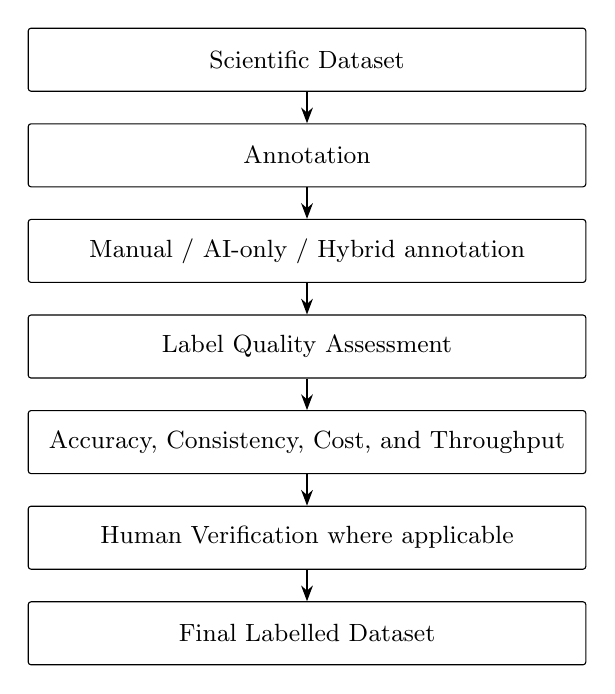
\begin{tikzpicture}[
  node distance=4mm,
  >={Stealth[length=2mm]},
  every node/.style={font=\small, align=center},
  workflow/.style={draw, rectangle, rounded corners=1pt, text width=68mm, minimum height=8mm, inner sep=4pt},
  link/.style={draw, ->, line width=0.45pt}
]
  \node[workflow] (dataset) {Scientific Dataset};
  \node[workflow, below=of dataset] (annotation) {Annotation};
  \node[workflow, below=of annotation] (approaches) {Manual / AI-only / Hybrid annotation};
  \node[workflow, below=of approaches] (quality) {Label Quality Assessment};
  \node[workflow, below=of quality] (criteria) {Accuracy, Consistency, Cost, and Throughput};
  \node[workflow, below=of criteria] (verification) {Human Verification where applicable};
  \node[workflow, below=of verification] (final) {Final Labelled Dataset};

  \draw[link] (dataset) -- (annotation);
  \draw[link] (annotation) -- (approaches);
  \draw[link] (approaches) -- (quality);
  \draw[link] (quality) -- (criteria);
  \draw[link] (criteria) -- (verification);
  \draw[link] (verification) -- (final);
\end{tikzpicture}
\caption{General workflow for scientific data labelling and quality assessment.}
\Description{A workflow beginning with a scientific dataset, followed by annotation, selection of manual, AI-only, or hybrid annotation, label quality assessment, evaluation of accuracy, consistency, cost, and throughput, human verification where applicable, and a final labelled dataset.}
\label{fig:annotation_workflow}
\end{figure}

\begin{itemize}
    \item \textbf{Systematic-review screening.} Multiple groups now use LLMs for title-and-abstract screening as an adjunct or filter ahead of human review. \citet{khraisha2023large} evaluated GPT-4 on peerreviewed and grey literature across multiple languages; the validation study of Llama 3 and ChatGPT-4o mini \citetext{PMC12623132} reports sensitivity/specificity trade-offs at the article level; and \citet{chen2025human} implement an explicit human-LLM collaboration protocol for randomizedcontrolled-trial screening in precision oncology, reporting improved reliability over unassisted GPT-3.5 screening.

    \item \textbf{Data extraction from full text.} \citet{mahmoudi2025critical} critically assess ChatGPT's performance extracting structured data fields from full-text articles for systematic reviews, an area where LLM outputs must be checked against source text because of documented risks of fabricated or inaccurate references and figures, as demonstrated by \citet{chelli2024hallucination} in their analysis of hallucination rates and reference accuracy for ChatGPT and Bard in systematic-review contexts.

    \item \textbf{Medical image and figure annotation.} \citet{dreizin2023accelerating} apply AI-collaborative labelling to CT trauma volumetry with explicit quality-assurance and bias-mitigation components; \citet*{chen2024quality} propose an automatic label-quality estimator (Quality Sentinel) applicable across 142 anatomical structures to flag both manual and AI-generated segmentation labels of doubtful quality; and \citet{yamagata2024survey} evaluate GPT-4 with vision for annotating cellular-senescence figures extracted from review articles, reporting over 70\% accuracy for label extraction and approximately 80\% accuracy for higher-level categorisation.

    \item \textbf{Metadata curation for data discovery.} \citet{turner2025large} apply GPT-4o to extract structured metadata (scanner parameters, participant characteristics, study design fields) from neuroimaging publications for the NeuroBridge data-discovery project, reporting agreement with human gold-standard annotation in the 0.91--0.97 range on several extraction sub-tasks.

    \item \textbf{Weakly and distantly supervised label induction for scientific documents.} Rather than using AI to check human labels, some pipelines induce labels automatically from structural cues in scientific documents themselves; \citet*{siegel2018extracting} generate over 5.5 million induced figure-extraction labels from arXiv and PubMed documents with no human annotation step, illustrating an alternative, fully automated route to large labelled scientific corpora where manual labelling at comparable scale would be impractical.

    \item \textbf{Cost-reduction infrastructure.} Commercial annotation platforms (e.g., Amazon SageMaker Ground Truth, Scale AI, and comparable tools referenced in recent dataset-safety literature for autonomous-driving perception data) now bundle semi-automated, machine-learning-assisted annotation with built-in quality-control mechanisms intended to preserve label accuracy and reliability while reducing per-label human effort, reflecting the same hybrid principle documented in the academic literature above.
\end{itemize}

\section{Research Challenges and Limitations}
\label{sec:challenges}

The existing evidence establishes that manual, AI-only, and hybrid annotation can each perform well under particular task conditions, but it does not yet support a single general ranking across scientific datasets. Five limitations constrain the conclusions that can be drawn: the lack of a stable ground truth, heterogeneity in tasks and evaluation methods, domain and language imbalance, limited measurement of reviewer behaviour, and the changing nature of proprietary models. These limitations define the unresolved problems that motivate the research directions in Section~\ref{sec:future-directions}.

\subsection{Absence of a stable ground truth}
\label{subsec:ground-truth}

A recurring methodological difficulty is that ``manual annotation'' is frequently treated as ground truth in comparative studies, even though the confident-learning literature demonstrates that manually curated benchmark test sets themselves contain pervasive label errors --- at least 3.3\% on average and as high as roughly 6\% for ImageNet's validation set (\citeauthor{northcutt2021pervasive}, 2021). Where multiple human experts disagree, majority voting has been shown not to reliably produce the best obtainable consensus, meaning that accuracy figures computed against any single human reference (or an unweighted panel) may misstate the true performance gap between AI-assisted and manual pipelines. The unresolved problem is therefore not only how to compare annotators, but how to construct a sufficiently reliable reference label against which manual, AI-only, and hybrid pipelines can all be evaluated fairly.

\subsection{Heterogeneity of tasks, models, and metrics}
\label{subsec:heterogeneity}

Reported accuracy figures are not directly comparable across studies because they span different tasks (text classification, image segmentation, figure annotation, metadata extraction), different models (GPT3.5, GPT-4, GPT-4o, Llama 3, and others), different prompting strategies (zero-shot versus few-shot versus fine-tuned), and different accuracy metrics (raw accuracy, sensitivity/specificity, Cohen's kappa, intercoder agreement). \citeauthor{delgadochaves2025large}'s reported 40--92\% accuracy range across 18 LLMs and three clinical domains illustrates how much of the apparent ``AI versus manual'' gap is really a product of model and prompt selection rather than a fixed property of AI assistance as such. Cost and accuracy are also commonly reported as separate headline outcomes, which prevents direct comparison at matched cost or matched accuracy. At the pipeline level, active-learning selection, AI pre-labelling, and human verification are more often evaluated as separate components than as a single integrated system. The unresolved problem is the absence of standardised, system-level evaluation that permits meaningful comparison across approaches.

\subsection{Domain and language imbalance in the evidence base}
\label{subsec:domain-language-imbalance}

Much of the strongest quantitative evidence for AI-assisted annotation accuracy comes from Englishlanguage biomedical systematic reviews and general social-media text classification. Studies in other scientific domains --- physical sciences, astronomy, materials science, and non-English scientific corpora --- are comparatively sparse, and where they exist, such as the Arabic discourse-annotation study by AlAthba and Zaghouani (2026), results can differ from the English biomedical literature, with manual annotation retaining a clearer advantage on culturally and linguistically nuanced material. Consequently, findings from the dominant English-language biomedical evidence base cannot be assumed to transfer unchanged to other scientific disciplines, languages, or culturally dependent annotation tasks. The unresolved problem is the limited external validity of the current comparisons.

\subsection{Automation bias and reviewer behaviour are under-measured}
\label{subsec:reviewer-behaviour}

Although automation bias is widely discussed as a risk of AI-assisted labelling pipelines, few of the peerreviewed studies reviewed here directly measure how reviewer verification behaviour changes when confronted with a pre-filled AI label versus a blank field, as opposed to simply reporting final accuracy after verification. This leaves an important causal question only partially answered: how much of any measured accuracy gain in hybrid pipelines is attributable to the AI system's raw suggestions being correct, versus to the review process itself catching errors, versus being offset by reviewers rubberstamping incorrect AI suggestions. Without separating these mechanisms, final hybrid-pipeline accuracy does not reveal whether human verification corrected model errors or merely confirmed model output. The unresolved problem is therefore causal attribution within the human--AI workflow.

\subsection{Reproducibility and versioning of proprietary models}
\label{subsec:reproducibility}

Because most of the strongest empirical results rely on proprietary, frequently updated commercial LLMs (ChatGPT/GPT-4-family models), accuracy figures reported at one point in time may not be reproducible with later model versions, and cost figures (e.g., the sub-cent per-annotation cost reported by Gilardi et al., 2023) can shift substantially as pricing and model architectures change, limiting the durability of quantitative benchmarks in this literature. A result tied to an incompletely specified model version, prompt, or evaluation date may therefore be difficult to reproduce or compare longitudinally. The unresolved problem is how to maintain durable evidence when the evaluated systems and their costs change over time.

\section{Research Gaps and Future Directions}
\label{sec:future-directions}

The research gaps below follow directly from the limitations in Section~\ref{sec:challenges}. Together, they move from weaknesses in the existing evidence to the unresolved methodological and empirical problems that future studies must address.

\begin{itemize}
    \item \textbf{Domain-diverse benchmarking.} To address the limited external validity of the current evidence, there is a clear need for large-scale, pre-registered comparisons of AI-assisted versus manual labelling accuracy across a wider range of genuinely scientific datasets --- physical sciences, environmental and earth sciences, astronomy, chemistry --- rather than the current concentration in biomedical text and imaging.

    \item \textbf{Causal decomposition of hybrid-pipeline gains.} To resolve uncertainty about reviewer behaviour, future work should experimentally separate the contribution of AI pre-labelling quality from the contribution of human verification behaviour (including automation bias), for example via randomized designs that vary whether reviewers see AI-suggested labels, blinded alternative labels, or no suggestion at all.

    \item \textbf{Better-than-majority-vote ground truth construction.} To overcome the absence of a stable reference standard, and building on findings that majority voting among experts is not always optimal, further methodological work is needed on principled ways to construct reference labels --- for example weighted consensus, expertise-adjusted aggregation, or confident-learning-style joint-distribution estimation --- against which both manual and AI-assisted pipelines can be fairly evaluated.

    \item \textbf{Standardised cost-accuracy reporting.} To make heterogeneous studies more comparable, and because cost and accuracy trade off differently across tasks, the field would benefit from standardised reporting of accuracy at matched cost (or cost at matched accuracy), rather than accuracy and cost reported as separate, non-comparable headline numbers.

    \item \textbf{Integrating active learning with AI-assisted verification.} To move from component-level evidence to system-level evaluation, future studies should directly evaluate pipelines that combine active-learning sample selection with AI-assisted pre-labelling and human verification as a single system, because relatively little published work evaluates the complete pipeline despite each component individually showing accuracy or efficiency benefits.

    \item \textbf{Longitudinal and versioning-aware evaluation.} To improve reproducibility as proprietary systems change, future studies should report results in a way that is explicit about model version and date, and ideally re-run key benchmarks periodically, to track whether the AI-assisted accuracy advantage over manual and crowd-based annotation is growing, stable, or task-dependent over time.

    \item \textbf{Non-English and low-resource scientific corpora.} To address the language imbalance in the evidence base, accuracy comparisons should be extended to non-English scientific literature and to low-resource languages, given evidence that current LLMs may underperform on culturally and linguistically nuanced annotation relative to trained human annotators in those settings.
\end{itemize}

\section{Conclusion}
\label{sec:conclusion}

The evidence reviewed here does not support a simple claim that AI-assisted labelling is categorically more or less accurate than manual labelling on scientific datasets. Instead, accuracy depends on task structure, model choice, and --- critically --- pipeline design. On well-defined classification and extraction tasks, AI assistance frequently matches or exceeds the accuracy of non-expert crowd annotation and, in several biomedical and neuroimaging studies, approaches the accuracy of trained human annotators. On tasks requiring deep contextual or cultural judgement, unaided manual annotation retains a measurable advantage. The most robust and consistently reported finding across the literature is that hybrid, humanin-the-loop pipelines --- in which AI systems generate candidate labels that trained humans verify and correct --- tend to outperform either pure approach in isolation, provided that automation bias is actively managed and the underlying model's baseline accuracy is sufficient to make verification worthwhile.

Because manually curated benchmark datasets themselves contain non-trivial label error, and because the evidence base remains concentrated in English-language biomedical and text-classification tasks, substantial further work is needed --- spanning broader scientific domains, more rigorous decomposition of where hybrid-pipeline accuracy gains come from, and standardised, cost-aware accuracy reporting --- before general conclusions about AI-assisted versus manual labelling accuracy can be drawn with confidence across the sciences as a whole.

\bibliographystyle{ACM-Reference-Format}
\bibliography{references}

\end{document}
